\chapter{Zero density energy theorems}


\begin{definition}[Zero density exponents]\label{zeroe-def}  For $1/2 \leq \sigma \leq 1$ and $T>0$, let $N^*(\sigma,T)$ denote the additive energy $E_1(\Sigma)$ of the imaginary parts of the zeroes $\rho$ of the Riemann zeta function with $\mathrm{Re}(\rho) \geq \sigma$ and $|\mathrm{Im}(\rho)| \leq T$.  For fixed $1/2 \leq \sigma \leq 1$, the zero density exponent $A^*(\sigma) \in [-\infty,\infty)$ is the infimum of all exponents $\A^*$ for which one has
    $$ N^*(\sigma-\delta,T) \ll T^{A^* (1-\sigma)+o(1)}$$
for all unbounded $T$ and infinitesimal $\delta>0$.
\end{definition}

The exponent $\A^*(\sigma)$ is also essentially referred to as $B(\sigma)$ in \cite{heath_brown_consecutive_II} (though without the technical shift by $\delta$ in that reference).


\begin{lemma}[Basic properties of $\A^*$]\label{zeroe-basic}\uses{zeroe-def}\
\begin{itemize}
\item[(i)] We have the trivial bounds
$$ 2\A(\sigma), 4\A(\sigma)-\frac{1}{1-\sigma} \leq \A^*(\sigma) \leq 3 \A(\sigma)$$
for any $1/2 \leq \sigma \leq 1$.
\item[(ii)] $\sigma \mapsto (1-\sigma) \A^*(\sigma)$ is non-increasing, with $\A^*(1/2)=6$ and $\A^*(1)=-\infty$.
\item[(iii)] If the Riemann hypothesis holds, then $\A^*(\sigma)=-\infty$ for all $1/2 < \sigma \leq 1$.
\end{itemize}
\end{lemma}

\derived 
\code{prove_heath_brown_energy_estimate()}
\begin{proof}\uses{add-energy, zero-basic} The claim (i) follows from Lemma \ref{add-energy}(iv), and the remaining claims then follow from Lemma \ref{zero-basic}.\end{proof}

Upper bounds on $\A^*(\sigma)$ can be obtained from large value energy theorems via the following relation.

\begin{lemma}[Zero density energy from large values energy]\label{zeroe-from-large}\uses{lvze-def}  Let $1/2 < \sigma < 1$.  Then
$$ \A^*(\sigma)(1-\sigma) \leq \max\left( \sup_{\tau \geq 1} \LV^*_\zeta(\sigma,\tau)/\tau, \limsup_{\tau \to \infty} \LV^*(\sigma,\tau)/\tau \right).$$
\end{lemma}

\begin{proof}\uses{lve-basic,zero-from-large,add-energy, lve-asymp}
Write the right-hand side as $B$, then $B \geq 0$ (from Lemma \ref{lve-basic}(iii)) and we have
\begin{equation}\label{lvze-bound}
    \LV^*_\zeta(\sigma,\tau) \leq B \tau
\end{equation}
for all $\tau \geq 1$, and
\begin{equation}\label{lve-bound}
    \LV^*(\sigma,\tau) \leq (B+\eps) \tau
\end{equation}
whenever $\eps>0$ and $\tau$ is sufficiently large depending on $\eps$ (and $\sigma$).  It would suffice to show, for any $\eps>0$, that $N^*(\sigma,T) \ll T^{B+O(\eps)+o(1)}$ as $T \to \infty$.

By dyadic decomposition, it suffices to show for large $T$ that the additive energy of imaginary parts of zeroes in $[T,2T]$ is $\ll T^{B+O(\eps)+o(1)}$.  As in the proof of Lemma \ref{zero-from-large}, we can assume the imaginary parts are $1$-separated (here we take advantage of the triangle inequality in Lemma \ref{add-energy}(iii)).

Suppose that one has a zero $\sigma'+i t$ of this form.  Then by standard approximations to the zeta function, one has
$$ \sum_{n \leq T} \frac{1}{n^{\sigma'+it}} \ll T^{-1}.$$
Let $0 < \delta_1 < \eps$ be a small quantity (independent of $T$) to be chosen later, and let $0 < \delta_2 < \delta_1$ be sufficiently small depending on $\delta_1,\delta_2$.  By the triangle inequality, and refining the sequence $t'$ by a factor of at most $2$, we either have
$$ \bigg|\sum_{T^{\delta_1} \leq n \leq T} \frac{1}{n^{\sigma'+it}} \bigg| \gg T^{-\delta_2}$$
for all zeroes, or \eqref{td}
for all zeroes.

Suppose we are in the former (``Type I'') case, we can dyadically partition and conclude from the pigeonhole principle that
$$ \bigg| \sum_{n \in I} \frac{1}{n^{\sigma'+it}} \bigg| \gg T^{-\delta_2-o(1)}$$
for some interval $I$ in some $[N,2N]$ with $T^{\delta_1} \ll N \ll T$, with at most $O(\log T)$ different choices for $I$.  Performing a Fourier expansion of $n^{\sigma'}$ in $\log n$ and using the triangle inequality one can then deduce that
$$ \bigg| \sum_{n \in I} \frac{1}{n^{it'}} \bigg| \gg N^{\sigma'} T^{-\delta_2-o(1)}$$
for some $t' = t + O(T^{o(1)})$; refining the $t$ by a factor of $T^{o(1)}$ if necessary, we may assume that the $t'$ are $1$-separated and that the interval $I$ is independent of $t'$, and by passing to a subsequence we may assume that $T = N^{\tau+o(1)}$ for some $1 \leq \tau \leq 1/\delta_1$, then
$$ \bigg| \sum_{n \in I} \frac{1}{n^{it'}} \bigg| \gg N^{\sigma-\delta_2/\delta_1+o(1)}$$
for all $t'$.  If we let $\Sigma'$ denote the set of such $t'$, then by Definition \ref{lvze-def} we then have (for $\delta_2$ small enough) we have
$$ E_1(\Sigma') \ll N^{\LV^*_\zeta(\sigma,\tau) + \eps + o(1)} \ll T^{\LV^*_\zeta(\sigma,\tau)/\tau + \eps + o(1)}.$$
By Lemma \ref{add-energy}(i) this implies that the set $\Sigma$ of real parts of zeroes under consideration also obeys the bound
$$ E_1(\Sigma) \ll T^{\LV^*_\zeta(\sigma,\tau)/\tau + \eps + o(1)}.$$
and the claim follows in this case from \eqref{lvze-bound}.

The Type II case similarly follows from \eqref{lve-bound} exactly as in the proof of Lemma \ref{zero-from-large}.
\end{proof}


\begin{corollary}\label{zeroe-large-cor-0}\uses{zeroe-def, lvze-def} Let $1/2 < \sigma < 1$ and $\tau_0 > 0$ be fixed.  Then
$$ \A^*(\sigma)(1-\sigma) \leq \max \left(\sup_{2 \leq \tau < \tau_0} \LV^*_\zeta(\sigma,\tau)/\tau, \sup_{\tau_0 \leq \tau \leq 2\tau_0} \LV^*(\sigma,\tau)/\tau\right)$$
\end{corollary}

\begin{proof}  Repeat the proof of Corollary \ref{zero-large-cor-0}.
\end{proof}

\begin{proposition}[Additive energy under the Lindelof hypothesis]\label{zeroe-lindelof}\uses{zeroe-def}  Let $1/2 \leq \sigma \leq 1$ be fixed.  Then one has
    $$ \A^*(\sigma) \leq 8 - 4\sigma$$
    and $\A^*(\sigma) \leq 0$ if $\sigma > 3/4$.
\end{proposition}

\begin{proof} See \cite[Lemma 4]{heath_brown_consecutive_II}.
\end{proof}

\begin{theorem}[Heath-Brown's additive energy bound]\label{hb-energy-bound}\cite[Theorem 2]{heathbrown_zero_1979}\uses{zeroe-def}  Let $1/2 \leq \sigma \leq 1$ be fixed.  Then one can bound $A^*(\sigma)$ by
    \begin{align*}
        \frac{10-11\sigma}{(2-\sigma)(1-\sigma)} & \hbox{ for } 1/2 \leq \sigma \leq 2/3;\\
        \frac{18-19\sigma}{(4-2\sigma)(1-\sigma)} & \hbox{ for } 2/3 \leq \sigma \leq 3/4;\\
        \frac{12}{4\sigma-1} & \hbox{ for } 3/4 \leq \sigma \leq 1.
    \end{align*}
\end{theorem}

\begin{proof}\uses{zeroe-large-cor-0, power-energy, hb-energy-simp, l2-mvt, hb-density, zeroe-basic, lvz-basic} We first suppose that $\sigma \leq 3/4$.  Here we apply Corollary \ref{zeroe-large-cor-0} with $\tau_0 = 2$.  The $\LV^*_\zeta$ supremum is now trivial, so it suffices to show that
\begin{equation}\label{second-claim}
        \rho^* \leq \max\left( \frac{10-11\sigma}{2-\sigma}, \frac{18-19\sigma}{4-2\sigma}\right) \tau
\end{equation}
whenever $(\sigma,\tau,\rho,\rho^*,s) \in \Energy$ with $2 \leq \tau \leq 3$.  Let $k$ be the first integer for which $1 \leq \tau/k \leq 3/2$, thus $k=2,3$ and also $\tau/(k+1) \leq 1$.  By Lemma \ref{power-energy}, there exist tuples
\begin{equation}\label{smak}
\left(\sigma, \frac{\tau}{k}, \rho', \frac{\rho^*}{k}, s'\right), \left(\sigma,\frac{\tau}{k+1}, \rho'', \frac{\rho^*}{k + 1}, s''\right)  \in \Energy.
\end{equation}
for some $\rho'$, $s'$, $\rho''$ and $s''$ satisfying
\[
\rho' \le \frac{\rho}{k},\qquad s' \le \frac{s}{k},\qquad \rho'' \le \frac{\rho}{k+1},\qquad s'' \le \frac{s}{k+1}.
\]
Applying Corollary \ref{hb-energy-simp} to the former tuple of \eqref{smak} and using $\rho' \le \rho/k$, we have
$$\frac{\rho^*}{k} \leq \max \left(\frac{3\rho}{k} + 1-2\sigma, \frac{\rho}{k} +4-4\sigma, \frac{5\rho}{2k} + \frac{3-4\sigma}{2}\right).$$
Write $\tau' := \tau/k$. Applying Lemma \ref{l2-mvt} to the first tuple of \eqref{smak} one has
$$\rho/k \leq \tau' + 1 - 2\sigma$$
while applying Lemma \ref{l2-mvt} to the second tuple of \eqref{smak} (recalling that $\tau/(k+1) \le 1$) gives
$$\rho/k = \frac{k+1}{k} \frac{\rho}{k+1} \leq \frac{k+1}{k} (2-2\sigma) \le 3-3\sigma$$
and thus
\begin{equation}\label{rho-k}
\rho/k \leq \min( \tau'+1-2\sigma, 3-3\sigma)
\end{equation}
and
\begin{equation*}
    \begin{split}
        \rho^*/k \leq \max(&3 \min(\tau'+1-2\sigma,3-3\sigma) + 1-2\sigma, \\
        &\min(\tau'+1-2\sigma,3-3\sigma) +4-4\sigma, \\
        &5\min(\tau'+1-2\sigma,3-3\sigma)/2 + (3-4\sigma)/2).
    \end{split}
\end{equation*}
A tedious calculation shows that for $1 \leq \tau' \leq 3/2$, we have
$$3 \min(\tau'+1-2\sigma,3-3\sigma) + 1-2\sigma \leq \frac{10-11\sigma}{2-\sigma} \tau',$$
$$ \min(\tau'+1-2\sigma,3-3\sigma) +4-4\sigma \leq \max\left( \frac{7-7\sigma}{2-\sigma}, 6-6\sigma\right)\tau'$$
and
$$5\min(\tau'+1-2\sigma,3-3\sigma)/2 + (3-4\sigma)/2 \leq \frac{18-19\sigma}{4-2\sigma} \tau'.$$
Since
$$\max\left( \frac{7-7\sigma}{2-\sigma}, 6-6\sigma\right) \leq \max\left(\frac{10-11\sigma}{2-\sigma}, \frac{18-19\sigma}{4-2\sigma}\right)$$
we obtain the claim.

Now suppose that $\sigma > 3/4$.  From Theorem \ref{hb-density} and Lemma \ref{zeroe-basic}(i) we are already done when $\sigma \geq 25/28$, so we may assume $\sigma < 25/28$.

Here we apply Corollary \ref{zeroe-large-cor-0} with $\tau_0 = 4\sigma-1$.  To control the $\LV^*_\zeta$ term, we need to establish
\begin{equation}\label{first-claim}
    \rho^* \leq \frac{12(1-\sigma)}{4\sigma-1} \tau
\end{equation}
whenever $(\sigma,\tau,\rho,\rho^*,s) \in \Energy_\zeta$ and $2 \leq \tau < 4\sigma-1$. We use Lemma \ref{lvz-basic}(ii) followed by Lemma \ref{hb-12} to give
$$ \rho^* \leq 3\rho \leq 3( 2\tau - 12 (\sigma-1/2) )$$
so the claim reduces to verifying
$$ 3( 2\tau - 12 (\sigma-1/2) ) \leq \frac{12(1-\sigma)}{4\sigma-1} \tau.$$
This holds with equality when $\tau = 4\sigma-1$, and the slope in $\tau$ is higher on the left-hand side for $\sigma>1/2$, so the claim \eqref{first-claim} follows.

It remains to establish
\begin{equation}\label{second-claim'}
    \rho^* \leq \frac{12(1-\sigma)}{4\sigma-1} \tau
\end{equation}
whenever $(\sigma,\tau,\rho,\rho^*,s) \in \Energy$ and $4\sigma-1 \leq \tau \leq 2(4\sigma-1)$.
Let $k$ be the first integer for which $(4\sigma-1)/2 \leq \tau/k \leq 3(4\sigma-1)/4$, thus $k=2,3$ and also $\tau/(k+1) \leq 4\sigma-1$.  By Lemma \ref{power-energy}, we have \eqref{smak}.
From Theorem \ref{huxley-lv} we have
$$\rho/k \leq \max(2-2\sigma, \tau' + 4 - 6\sigma)$$
and also
$$\rho/k = \frac{k+1}{k} \frac{\rho}{k+1} \leq \frac{k+1}{k} (2-2\sigma) \le 3-3\sigma$$
and hence
\begin{equation}\label{rhok} \rho/k \leq \min( \max(2-2\sigma, \tau' + 4 - 6\sigma), \tau'+4-6\sigma, 3-3\sigma).
\end{equation}
Among other things, this implies that $\rho/k \leq 1$.

From Theorem \ref{hbt} and $\rho' \le \rho/k$, we have
\begin{equation}\label{rhok-star}
\begin{split}
\rho^*/k \leq 1-2\sigma &+ \frac{1}{2}\max\left(\frac{\rho}{k}+1, \frac{2\rho}{k}, \frac{5\rho}{4k} + \frac{\tau'}{2}\right)\\
&+ \frac{1}{2}\max\left(\frac{\rho^*}{k}+1, \frac{4\rho}{k}, \frac{3\rho^*}{4k}+\frac{\rho}{k}+\frac{\tau'}{2}\right)
\end{split}
\end{equation}
where $\tau' := \tau/k$.  This expression is complicated, so we divide into cases.
First suppose that $\rho/k+1 \geq 5\rho/4k + \tau'/2$.  In this case the first maximum in the above expression is $\rho/k+1$, and we simplify to
$$ \rho^*/k \leq 3/2-2\sigma + \rho/2k + \max(\rho^*/k+1, 4\rho/k, 3\rho^*/4k+\rho/k+\tau'/2)/2,$$
which after solving for $\rho^*/k$ gives
$$ \rho^*/k \leq \max( \rho/2k + 4-4\sigma, 5\rho/2k + (3-4\sigma)/2, 8\rho/5k + 2\tau'/5 + (12-16\sigma)/5).$$
Inserting \eqref{rhok}, one can verify after a tedious analysis (using the hypothesis $3/4 \leq \sigma < 25/28$) that
\begin{equation}\label{rhost}
    \rho^*/k \leq \frac{12(1-\sigma)}{4\sigma-1} \tau'
\end{equation}
as required.

It remains to treat the case where $\rho/k+1 > 5\rho/4k + \tau'/2$.  Using \eqref{rhok} one can check that this forces
\begin{equation}\label{4s}
    4\sigma-2 \leq \tau' \leq \frac{3}{4}(4\sigma-1),
\end{equation}
so that \eqref{rhok} now becomes
\begin{equation}\label{rhok-simp}
\rho/k \leq 3-3\sigma.
\end{equation}
The bound \eqref{rhok-star} becomes
$$\rho^*/k \leq 1-2\sigma + (5\rho/4k+\tau'/2)/2 + \max(\rho^*/k+1, 4\rho/k, 3\rho^*/4k+\rho/k+\tau'/2)/2$$
which simplifies to
$$ \rho^*/k \leq \max( 5\rho/4k + \tau'/2 + 3-4\sigma, 21\rho/8k + \tau'/4 + 1-2\sigma, 9\rho/5k + 4\tau'/5 + (8 - 16\sigma)/5).$$
Inserting \eqref{rhok-simp} and \eqref{4s}, one can eventually show (again using the hypothesis $3/4 \leq \sigma < 25/28$) that
\eqref{rhost} holds as required.
\end{proof}

We found the following estimates with the aid of computer assistance, which improve on Theorem \ref{hb-energy-bound} in various ranges of $\sigma$. 
\begin{theorem}\label{imp-hb-energy-bound}
For $3/4 \le \sigma \le 5/6$ one has 
\[
\A^*(\sigma) \le \min\left(\frac{18 - 19\sigma}{2(3\sigma - 1)(1-\sigma)}, \frac{4(10 - 9\sigma)}{5(4\sigma - 1)(1 - \sigma)}\right).
\]
\end{theorem}

\derived 
\code{prove_improved_heath_brown_energy_estimate()}

\begin{proof}
Throughout assume that $3/4 \le \sigma \le 5/6$. Choose 
\[
\tau_0 = 8\sigma - 4.
\]
We will show that
\begin{equation}\label{imphb_lver_ineq}
\rho^* \le \begin{cases}
\dfrac{18 - 19\sigma}{2(3\sigma - 1)},&3/4 \le \sigma < 4/5\\
\dfrac{7(1 - \sigma)}{3\sigma - 1},&4/5 \le \sigma \le 5/6,
\end{cases} 
\end{equation}
for all $(\sigma, \tau, \rho, \rho^*, s) \in \Energy$ for which $\tau_0 \le \tau \le 2\tau_0$, and that
\begin{equation}\label{imphb_zlver_ineq}
\rho^* \le \begin{cases}
\dfrac{45 - 46\sigma}{4(4\sigma - 1)}\tau,&3/4 \le \sigma < 65/86,\\
\dfrac{4(10 - 9\sigma)}{5(4\sigma - 1)}\tau,&65/86 \le \sigma \le 5/6.
\end{cases}
\end{equation}
for all $(\sigma, \tau, \rho, \rho^*, s) \in \Energy_\zeta$ such that $2 \le \tau \le \tau_0$. The desired result then follows from computing the piecewise maximum of \eqref{imphb_lver_ineq} and \eqref{imphb_zlver_ineq}. 

First, consider \eqref{imphb_zlver_ineq}. Suppose that $(\sigma, \tau, \rho, \rho^*, s)\in \Energy_\zeta$ with $3/4 \le \sigma \le 5/6$ and $2 \le \tau \le \tau_0$. Then, from Theorem \ref{hb-12},
\begin{equation}\label{hb-lv-rho-form}
\rho \le 2\tau - 12(\sigma - 1/2).
\end{equation}
Furthermore, by Theorem \ref{huxley-lv} and Lemma \ref{power-lemma} with $k = 2$, one has $\rho \le 2\max(2 - 2\sigma, 4 - 6\sigma + \tau/2)$. However since $\tau \le \tau_0 = 8\sigma - 4$, this simplifies to 
\begin{equation}
\label{huxley_lv_rho_form2}
\rho \le 4 - 4\sigma.
\end{equation}
Since $\sigma \ge 3/4$, this also implies that $\rho \le 1$. For future reference we also note that 
\begin{equation}\label{zlver:tau_gradient_1}
1 < \frac{45 - 46\sigma}{4(4\sigma - 1)} < 2,\qquad (3/4 \le \sigma \le 65/86),
\end{equation}
\begin{equation}\label{zlver:tau_gradient_2}
\frac{6}{7} \le \frac{4(10 - 9\sigma)}{5(4\sigma - 1)} < 2,\qquad (65/86 \le \sigma \le 5/6).
\end{equation}
By Theorem \ref{power-lemma}, one has
\[
\rho^* \leq 1-2\sigma + \frac{1}{2}\max(\rho+1, 2\rho, \frac{5}{4}\rho+\frac{\tau}{2}) + \frac{1}{2}\max(\rho^*+1, 4\rho, \frac{3}{4}\rho^*+\rho+\frac{\tau}{2})
\]
Since $\rho \le 1$, one has $\rho + 1 \ge 2\rho$. Thus the middle term in the first maximum may be omitted, and we are left with two cases to consider. 

\textbf{Case 1:} If $\rho + 1 \ge 5\rho/4 + \tau/2$ then 
\[
\rho^* \le 1 -2\sigma + \frac{\rho + 1}{2} + \frac{1}{2}\max(\rho^* + 1, 4\rho, \frac{3}{4}\rho^*+\rho +\frac{\tau}{2}).
\]
Solving for $\rho^*$ gives 
\[
\rho^* \le \max(4 - 4\sigma + \rho, \frac{3}{2} - 2\sigma + \frac{5}{2}\rho, \frac{2}{5}(6 - 8\sigma + \tau + 4\rho)).
\]
Applying \eqref{huxley_lv_rho_form2} to each term,
\[
\rho^* \le M_1 := \max(8 - 8\sigma, \frac{23}{2} - 12\sigma, \frac{2}{5}(22 - 24\sigma + \tau)).
\]
For $3/4 \le \sigma \le 5/6$ and $\tau \ge 2$, one has 
\[
M_1 \le \frac{45 - 46\sigma}{4(4\sigma - 1)}\tau
\]
since by \eqref{zlver:tau_gradient_1}, each term in $M_1$ increases slower in $\tau$ than the RHS, and the inequality holds at $\tau = 2$. Similarly, one can verify that
\[
M_1 \le \frac{4(10 - 9\sigma)}{5(4\sigma - 1)}\tau
\]
for $65/86 \le \sigma \le 5/6$ and $\tau \ge 2$ (with some room to spare). 

\textbf{Case 2:} If $\rho + 1 < 5\rho/4 + \tau/2$, then  
\[
\rho^* \le 1 - 2\sigma + \frac{5}{8}\rho + \frac{\tau}{4} + \frac{1}{2}\max(\rho^* + 1, 4\rho, \frac{3}{4}\rho^*+\rho +\frac{\tau}{2})
\]
Solving for $\rho$ gives 
\[
\rho^* \le \max(3 - 4\sigma + \frac{\tau}{2} + \frac{5}{4}\rho, 1 - 2\sigma + \frac{\tau}{4} + \frac{21}{8}\rho, \frac{8 - 16\sigma + 4\tau + 9\rho}{5})
\]
If $\tau \ge 4\sigma - 1$, then apply \eqref{huxley_lv_rho_form2} termwise to get 
\[
\rho^* \le M_2 := \max(8 - 9\sigma + \frac{\tau}{2}, \frac{23}{2} - \frac{25}{2} + \frac{\tau}{4}, \frac{4}{5}(11 - 13 \sigma + \tau)).
\]
For $3/4 \le \sigma \le 65/86$ and $\tau \ge 4\sigma - 1$ one has 
\[
M_2 \le \frac{45 - 46\sigma}{4(4\sigma - 1)}\tau
\]
since by \eqref{zlver:tau_gradient_2} each term in $M_2$ is growing slower in $\tau$ than the RHS, and at $\tau = 4\sigma - 1$ we have equality. Similarly, one may verify that $M_2 \le 4(10 - 9\sigma)/(5(4\sigma - 1))\tau$ for $65/86 \le \sigma \le 5/6$ and $\tau \ge 4\sigma - 1$. 

On the other hand if $\tau < 4\sigma - 1$ then we apply \eqref{hb-lv-rho-form} termwise to get 
\[
\rho^* \le M_3 := \max(\frac{21}{2} - 19\sigma + 3\tau, \frac{67 -134\sigma + 22\tau}{4}, \frac{2}{5}(31 - 62\sigma + 11\tau)).
\]
Similarly to before, if $3/4 \le \sigma \le 65/86$ and $\tau < 4\sigma - 1$ then 
\[
M_3 < \frac{45 - 46\sigma}{4(4\sigma - 1)}\tau
\]
since each term in $M_3$ is growing faster in $\tau$ than the RHS, and at $\tau = 4\sigma - 1$ one has equality. Similarly, one may verify that $M_3 \le 4(10 - 9\sigma)/(5(4\sigma - 1))\tau$ for $65/86 \le \sigma \le 5/6$ and $\tau < 4\sigma - 1$. 

Thus we have shown that if $(\sigma, \tau, \rho, \rho^*, s) \in \Energy_\zeta$ with $3/4 \le \sigma \le 5/6$ and $2 \le \tau \le 8\sigma - 4$, then 
\[
\rho^*/\tau \le \min\left(\frac{45 - 46\sigma}{4(4\sigma - 1)}, \frac{4(10 - 9\sigma)}{5(4\sigma - 1)}\right).
\]

Now consider \eqref{imphb_lver_ineq}. Suppose that $\tau_0 \le \tau \le 2\tau_0$ and $(\sigma, \tau, \rho, \rho^*, s) \in \Energy$. Note that the interval $[\tau_0, 2\tau_0]$ is covered by intervals $I_k := [(4\sigma - 2)k, (4\sigma - 2)(k + 1)]$ with $k = 2, 3$. Suppose that $\tau \in I_k$. Then, by Theorem \ref{huxley-lv} and $\tau \ge (4\sigma - 2)k$ one has
\[
\rho/k \le \max(2 - 2\sigma, 4 - 6\sigma + \tau/k) = 4 - 6\sigma + \tau/k.
\]
Also, from Theorem \ref{huxley-lv} and $\tau \le (4\sigma - 2)(k + 1)$ one has
\[
\rho/(k + 1) \le \max(2 - 2\sigma, 4 - 6\sigma + \tau/(k + 1)) \le 2 - 2\sigma.
\]
In summary,
\begin{equation}\label{ze_ihb_rho_bound_k}
\rho/k \le \min((2 - 2\sigma)\frac{k + 1}{k}, 4 - 6\sigma + \frac{\tau}{k}).
\end{equation}
In particular, this implies that $\rho/k \le 1$ since $\sigma \ge 3/4$ implies $3 - 3\sigma < 1$.

We also note for future use that 
\begin{equation}\label{ze_ihb_bound_tau_factor}
1 \le \frac{18 - 19\sigma}{6\sigma - 2} \le \frac{3}{2}.
\end{equation}
Next, by Lemma \ref{power-energy}, 
\[
(\sigma, \tau', \rho', \rho^*/k, s') \in \Energy
\]
for $\tau' := \tau/k$ and some $\rho' \le \rho/k$ and $s' \le s/k$. 

Applying Lemma \ref{hbt} to this tuple, then apply $\rho' \le \rho/k$:
\[
\rho^*/k \leq 1-2\sigma + \frac{1}{2}\max(\frac{\rho}{k}+1, \frac{2\rho}{k}, \frac{5\rho}{4k} + \frac{\tau'}{2}) + \frac{1}{2}\max(\frac{\rho^*}{k}+1, \frac{4\rho}{k}, \frac{3}{4}\frac{\rho^*}{k} +\frac{\rho}{k}+\frac{\tau'}{2})
\]
Since $\rho/k \le 1$ there are only two cases to consider:

\textbf{Case 1:} $\rho/k + 1 \ge 5\rho/(4k) + \tau'/2$ then 
\[
\frac{\rho^*}{k} \le \frac{3}{2} - 2\sigma + \frac{\rho}{2k} + \frac{1}{2}\max(\frac{\rho^*}{k}+1, \frac{4\rho}{k}, \frac{3}{4}\frac{\rho^*}{k} +\frac{\rho}{k}+\frac{\tau'}{2})
\]
Solving for $\rho^*/k$, we get 
\[
\rho^*/k \le \max(4(1 - \sigma) + \frac{\rho}{k}, \frac{(3 - 4\sigma) + 5\rho/k}{2}, \frac{2}{5}((6 - 8\sigma) + \tau' + \frac{4\rho}{k}))
\]
If $4\sigma - 2 + 2(1 - \sigma)/k \le \tau' \le (4\sigma - 2)(k + 1)/k$ then by applying $\rho/k \le (2 - 2\sigma)(k + 1)/k$ from \eqref{ze_ihb_rho_bound_k}, one has
\[
\rho^*/k \le \max((6 + \frac{2}{k})(1 - \sigma), \frac{13}{2} - 7\sigma + \frac{5}{k} (1 - \sigma), \frac{2}{5}(14 - 16\sigma + \tau' + \frac{8}{k}(1 - \sigma)))
\]
However for $3/4 \le \sigma \le 4/5$, $k \ge 2$ and $\tau' \ge 4\sigma - 2 + 2(1 - \sigma)/k$ one has  
\begin{align*}
\frac{18 - 19\sigma}{6\sigma - 2}\tau' - (6 + \frac{2}{k})(1 - \sigma) &\ge \frac{18 - 19\sigma}{6\sigma - 2}(4\sigma - 2 + \frac{2}{k}(1 - \sigma)) - (6 + \frac{2}{k})(1 - \sigma) \\
&= \frac{(4 - 5\sigma) ((4\sigma - 3)k - 5\sigma + 5)}{k(3\sigma - 1)} \ge 0,
\end{align*}
\begin{align*}
&\frac{18 - 19\sigma}{6\sigma - 2}\tau' - \left(\frac{13}{2} - 7\sigma + \frac{5}{k} (1 - \sigma)\right) \\
&\qquad\ge \frac{18 - 19\sigma}{6\sigma - 2}(4\sigma - 2 + \frac{2}{k}(1 - \sigma)) - \left(\frac{13}{2} - 7\sigma + \frac{5}{k} (1 - \sigma)\right) \\
&\qquad= \frac{(k - 2) (34\sigma - 23) (1 - \sigma)}{2 k (3\sigma - 1)} \ge 0,
\end{align*}
\begin{align*}
&\frac{18 - 19\sigma}{6\sigma - 2}\tau' - \frac{2}{5}(14 - 16\sigma + \tau' + \frac{8}{k}(1 - \sigma)) \\
&\qquad\ge \left(\frac{18 - 19\sigma}{6\sigma - 2} - \frac{2}{5}\right)(4\sigma - 2 + \frac{2}{k}(1 - \sigma)) - \frac{2}{5}(14 - 16\sigma + \frac{8}{k}(1 - \sigma))\\
&\qquad= \begin{cases}
(22 - 27\sigma)/10,&k = 2,\\
(88 - 272\sigma + 199\sigma^2)/(15(1 - 3\sigma)),&k=3,
\end{cases}\\
&\qquad\ge 0. 
\end{align*}
Therefore 
\begin{equation}\label{ze_ihb_rhok_targetbound}
\rho^*/k \le \frac{18 - 19\sigma}{6\sigma - 2}\tau'
\end{equation}
in this case. 

On the other hand, if $4\sigma - 2 \le \tau' \le 4\sigma - 2 + 2(1 - \sigma)/k$ then applying $\rho/k \le 4 - 6\sigma + \tau'$ one has 
\[ 
\rho^*/k \le \max(8 -10\sigma + \tau',\frac{23 - 34\sigma + 5\tau'}{2}, \frac{2}{5}(22 - 32\sigma +  5\tau'))
\]
Similarly to before, for $3/4 \le \sigma \le 4/5$ and $4\sigma - 2 \le \tau' \le 4\sigma - 2 + 2(1 - \sigma)/k$ one has (in view of \eqref{ze_ihb_bound_tau_factor})
\begin{align*}
\frac{18 - 19\sigma}{6\sigma - 2}\tau' - (8 - 10\sigma + \tau') &\ge \left(\frac{18 - 19\sigma}{6\sigma - 2} - 1\right)(4\sigma - 2) - (8 - 10\sigma) \\
&= \frac{20}{3}\frac{(\sigma - 3/4) (4/5 - \sigma)}{\sigma - 1/3} \ge 0,
\end{align*}
\begin{align*}
\frac{18 - 19\sigma}{6\sigma - 2}\tau' - \frac{23 - 34\sigma + 5\tau'}{2} &\ge \left(\frac{18 - 19\sigma}{6\sigma - 2} - \frac{5}{2}\right)(4\sigma - 2 + \frac{2}{k}(1 - \sigma)) - \frac{23 - 34\sigma}{2}\\
&= \frac{(k - 2)(34\sigma - 23)(1 - \sigma)}{2k(3\sigma - 1)} \ge 0,
\end{align*}
\begin{align*}
\frac{18 - 19\sigma}{6\sigma - 2}\tau' - \frac{2}{5}(22 - 32\sigma +  5\tau') &\ge \left(\frac{18 - 19\sigma}{6\sigma - 2} - 2\right)(4\sigma - 2 + \frac{2}{k}(1 - \sigma)) - \frac{2}{5}(22 - 32\sigma)\\
&= \begin{cases}
(22 - 27\sigma)/10,&k = 2,\\
(88 - 272\sigma + 199\sigma^2)/(15(1 - 3\sigma)),&k=3,
\end{cases}\\
&\ge 0. 
\end{align*}
Therefore, \eqref{ze_ihb_rhok_targetbound} holds in this case too.

\textbf{Case 2:} $\rho/k + 1 < 5\rho/(4k) + \tau'/2$ then 
\[
\rho^*/k \leq 1-2\sigma + \frac{5\rho}{8k} + \frac{\tau'}{4} + \frac{1}{2}\max(\frac{\rho^*}{k}+1, \frac{4\rho}{k}, \frac{3}{4}\frac{\rho^*}{k} + \frac{\rho}{k}+\frac{\tau'}{2})
\]
Solving for $\rho^*/k$ gives 
\[
\rho^*/k \le \max(3 - 4\sigma + \frac{\tau'}{2} + \frac{5}{4}\frac{\rho}{k}, 1 - 2\sigma + \frac{\tau'}{4} + \frac{21}{8}\frac{\rho}{k}, \frac{1}{5}(8 - 16\sigma + 4\tau' + 9\frac{\rho}{k}))
\]
Proceeding as before, if $4\sigma - 2 + 2(1 - \sigma)/k \le \tau' \le (4\sigma - 2)(k + 1)/k$ then by applying $\rho/k \le (2 - 2\sigma)(k + 1)/k$ from \eqref{ze_ihb_rho_bound_k}, one has
\begin{align*}
\rho^*/k \le \max(&\frac{11 - 13\sigma + \tau' + 5(1 - \sigma)/k}{2}, \frac{25 - 29\sigma + \tau' + 21(1-\sigma)/k}{4},\\
&\qquad\frac{2}{5}(13 - 17 \sigma + 2\tau' + 9 (1 - \sigma)/k))
\end{align*}
Via a similar argument to before, using \eqref{ze_ihb_bound_tau_factor} and $\tau' \ge 4\sigma - 2 + 2(1 - \sigma)/k$ one eventually obtains, for $3/4 \le \sigma \le 4/5$,
\[
\frac{18 - 19\sigma}{6\sigma - 2}\tau' - \frac{11 - 13\sigma + \tau' + 5(1 - \sigma)/k}{2} \ge \begin{cases}
(11 - 13\sigma)/4,&k = 2\\
(44\sigma^2 - 60\sigma + 19)/(3 - 9\sigma),&k=3
\end{cases}\ge 0,
\]
\[
\frac{18 - 19\sigma}{6\sigma - 2}\tau' - \frac{25 - 29\sigma + \tau' + 21(1-\sigma)/k}{4} \ge \frac{(1 - \sigma) (95 - 49 k - (145 - 77 k)\sigma)}{4 k (3\sigma - 1)} \ge 0,
\]
\[
\frac{18 - 19\sigma}{6\sigma - 2}\tau' - \frac{2}{5}(13 - 17 \sigma + 2\tau' + 9(1 - \sigma)/k)) = \begin{cases}
(28 - 33\sigma)/10,&k = 2\\
(47\sigma^2 - 64\sigma + 20)/(3 - 9\sigma)&k=3
\end{cases}\ge 0.
\]
Thus also 
\[
\rho^*/k \le \frac{18 - 19\sigma}{6\sigma - 2}\tau'
\]
in this case. 

Similarly, if $(4\sigma - 2) \le \tau' \le 4\sigma - 2 + 2(1 - \sigma)/k$ then using $\rho/k \le 4 - 6\sigma + \tau'$ from \eqref{ze_ihb_rho_bound_k} one has
\[
\rho^*/k \le \max(8 - \frac{23\sigma}{2} + \frac{7\tau'}{4}, \frac{23}{2} - \frac{71\sigma}{4} + \frac{23\tau'}{8}, \frac{44 - 70\sigma + 13\tau'}{5})
\]
Via a similar argument as before, using \eqref{ze_ihb_bound_tau_factor} and $\tau' \le 4\sigma - 2 + 2(1 - \sigma)/k$ one ultimately obtains, for $3/4 \le \sigma \le 4/5$,
\[
\frac{18 - 19\sigma}{6\sigma - 2}\tau' - (8 - \frac{23\sigma}{2} + \frac{7\tau'}{4}) \ge \begin{cases}
(11 - 13 \sigma)/4,&k = 2\\
(44\sigma^2 - 60\sigma + 19)/(3 - 9\sigma),&k = 3
\end{cases} > 0,
\]
\[
\frac{18 - 19\sigma}{6\sigma - 2}\tau' - (\frac{23}{2} - \frac{71\sigma}{4} + \frac{23\tau'}{8}) \ge \frac{(1 - \sigma) (95 - 49 k - (145 - 77 k)\sigma)}{4 k (3\sigma - 1)} > 0,
\]
\[
\frac{18 - 19\sigma}{6\sigma - 2}\tau' - \frac{44 - 70\sigma + 13\tau'}{5} \ge \begin{cases}
(28 - 33\sigma)/10,&k = 2\\
(47\sigma^2 - 64\sigma + 20)/(3 - 9\sigma),&k=3
\end{cases} > 0.
\]
Combining all the cases, we have shown that $3/4 \le \sigma \le 4/5$ and $\tau_0 \le \tau' \le 2\tau_0$ one has 
\[
\rho^*/k \le \frac{18 - 19\sigma}{6\sigma - 2}\tau'
\]
from which the desired result follows. 

The case for $4/5 \le \sigma \le 5/6$ may be treated similarly. Here one may verify that 
\[
\max((6 + \frac{2}{k})(1 - \sigma), \frac{13}{2} - 7\sigma + \frac{5}{k} (1 - \sigma), \frac{2}{5}(14 - 16\sigma + \tau' + \frac{8}{k}(1 - \sigma))) \le \frac{7(1 - \sigma)}{3\sigma - 1}\tau',
\]
\[
\max(\frac{11 - 13\sigma + \tau' + 5(1 - \sigma)/k}{2}, \frac{25 - 29\sigma + \tau' + 21(1-\sigma)/k}{4},\frac{2}{5}(13 - 17 \sigma + 2\tau' + 9 (1 - \sigma)/k)) \le \frac{7(1 - \sigma)}{3\sigma - 1}\tau'
\]
for $4\sigma - 2 + 2(1 - \sigma)/k \le \tau' \le (4\sigma - 2)(k + 1)/k$, and that 
\[
\max(8 -10\sigma + \tau',\frac{23 - 34\sigma + 5\tau'}{2}, \frac{2}{5}(22 - 32\sigma +  5\tau')) \le \frac{7(1 - \sigma)}{3\sigma - 1}\tau',
\]
\[
\max(8 - \frac{23\sigma}{2} + \frac{7\tau'}{4}, \frac{23}{2} - \frac{71\sigma}{4} + \frac{23\tau'}{8}, \frac{44 - 70\sigma + 13\tau'}{5}) \le \frac{7(1 - \sigma)}{3\sigma - 1}\tau'
\]
for $4\sigma - 2 \le \tau' \le 4\sigma - 2 + 2(1 - \sigma)/k$. The treatment is analogous to before, so we omit the proof. 
\end{proof}


\begin{table}[ht]
    \def\arraystretch{2}
    \centering
    \caption{Current best upper bound on $\A(\sigma)$}
    \begin{tabular}{|c|c|c|}
    \hline
    $\A^*(\sigma)$ bound & Range & Reference\\
    \hline
    $\dfrac{10 - 11\sigma}{(2 - \sigma)(1 - \sigma)}$ & $\dfrac{1}{2} \leq \sigma \le \dfrac{2}{3} = 0.6666\ldots$ & Theorem \ref{hb-energy-bound}\\
    \hline
    $\dfrac{18 - 19\sigma}{(4 - 2\sigma)(1 - \sigma)}$ & $\dfrac{2}{3} \leq \sigma \le \dfrac{3}{4} = 0.75\ldots$ & Theorem \ref{hb-energy-bound}\\
    \hline
    $\dfrac{18 - 19\sigma}{(6\sigma - 2)(1 - \sigma)}$ & $\dfrac{3}{4} \leq \sigma \le \dfrac{143 + \sqrt{13889}}{328} = 0.7952\ldots$ & Theorem \ref{imp-hb-energy-bound}\\
    \hline
    $\dfrac{40 - 36\sigma}{(20\sigma - 5)(1 - \sigma)}$ & $\dfrac{143 + \sqrt{13889}}{328} \leq \sigma \le \dfrac{5}{6} = 0.8333\ldots$ & Theorem \ref{imp-hb-energy-bound}\\
    \hline
    $\dfrac{12}{4\sigma - 1}$ & $\dfrac{5}{6} \leq \sigma \le 1$ & Theorem \ref{hb-energy-bound}\\
    \hline
    \end{tabular}
    \label{zero_density_energy_estimates_table}
\end{table}

\begin{figure}
    \centering
    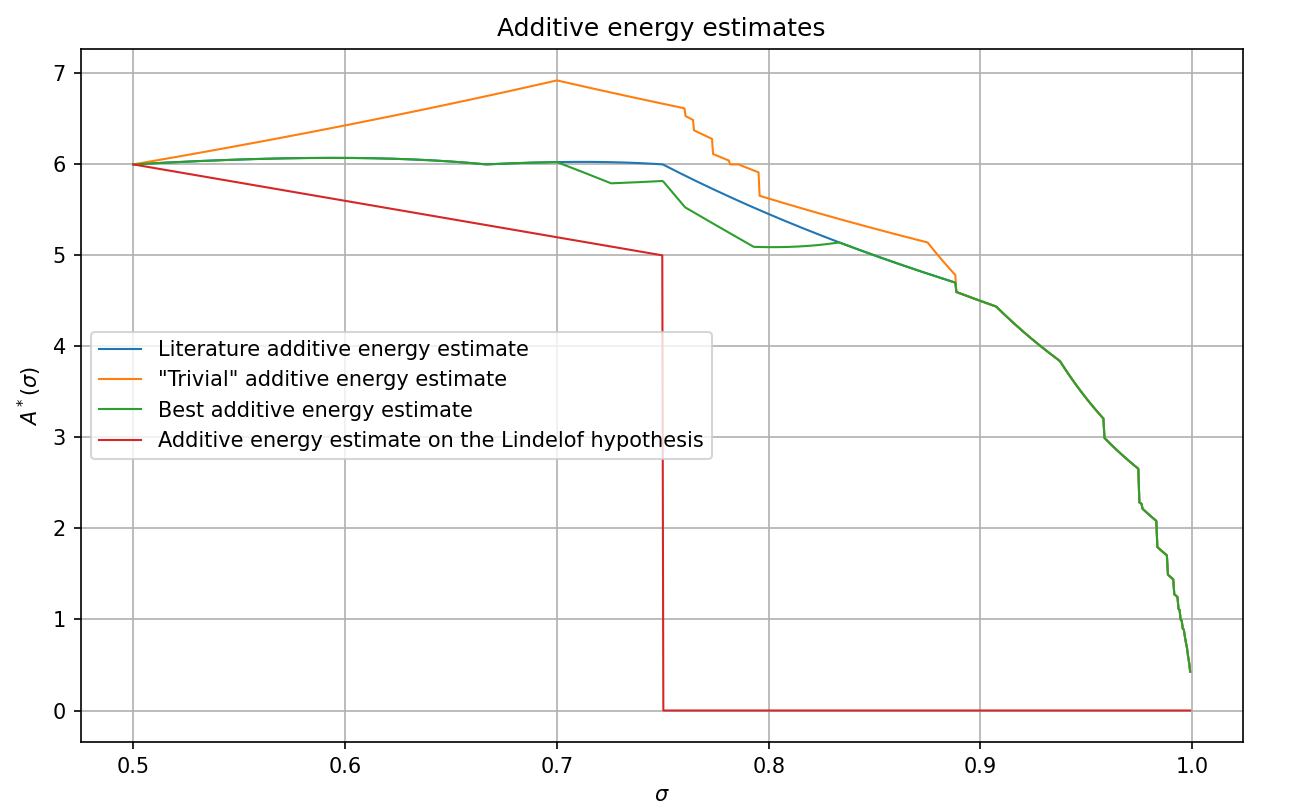
\includegraphics[width=0.5\linewidth]{chapter/zero_density_energy_estimate.png}
    \caption{Comparison of bounds on $\A^*(\sigma)$ under various assumptions.}
    \label{fig:zero_density_energy_estimate}
\end{figure}


